%!TeX encoding = UTF-8
%!TeX program = xelatex

\documentclass[notheorems, aspectratio=169]{beamer}
% aspectratio: 1610, 149, 54, 43(default), 32

% Input configuration
\usepackage[utf8]{inputenc}

% -- support vietnamese --
% \usepackage[vietnamese]{babel}
% -- support english --
\usepackage[english]{babel}
% ----------------------------------------------

% For math
\usepackage{amsmath,amssymb}
\usepackage{mathtools}
\usepackage{amsthm}
% \newcommand{\N}{\mathbb{N}}
% \newcommand{\Z}{\mathbb{Z}}
% \newcommand{\R}{\mathbb{R}}
% \newcommand{\F}{\mathbb{F}}
% ----------------------------------------------

% For images, colors
\usepackage{graphicx}
\usepackage{color,xcolor}
% ----------------------------------------------

% For captioning
\usepackage{caption}
\setbeamertemplate{caption}[numbered]
% ----------------------------------------------

% For tables
\usepackage{booktabs}
% ----------------------------------------------

% For hyper references between sections
\usepackage{hyperref}
% ----------------------------------------------

% For texts, algorithm and codes
\usepackage{ulem}
\usepackage{algorithm}
\usepackage{listings}
% ----------------------------------------------

% For tikz
\usepackage{framed}
\usepackage{tikz}
\usepackage{pgf}
\usetikzlibrary{calc,trees,positioning,arrows,chains,shapes.geometric,%
decorations.pathreplacing,decorations.pathmorphing,shapes,%
matrix,shapes.symbols}
\pgfmathsetseed{1} % To have predictable results
% Define a background layer, in which the parchment shape is drawn
\definecolor{doge}{HTML}{0065BD}
\pgfdeclarelayer{background}
\pgfsetlayers{background, main}

% Macro to draw the shape behind the text, when it fits completly in the page
% define styles for the normal border and the torn border
\tikzset{
  normal border/.style={doge!40!black!10, decorate, 
     decoration={random steps, segment length=2.5cm, amplitude=.7mm}},
  torn border/.style={doge!40!black!5, decorate, 
     decoration={random steps, segment length=.5cm, amplitude=1.7mm}}}

% Macro to draw the shape behind the text, when it fits completly in the
% page
\def\parchmentframe#1{
\tikz{
  \node[inner sep=2em] (A) {#1};  % Draw the text of the node
  \begin{pgfonlayer}{background}  % Draw the shape behind
  \fill[normal border] 
        (A.south east) -- (A.south west) -- 
        (A.north west) -- (A.north east) -- cycle;
  \end{pgfonlayer}}}

% Macro to draw the shape, when the text will continue in next page
\def\parchmentframetop#1{
\tikz{
  \node[inner sep=2em] (A) {#1};    % Draw the text of the node
  \begin{pgfonlayer}{background}    
  \fill[normal border]              % Draw the ``complete shape'' behind
        (A.south east) -- (A.south west) -- 
        (A.north west) -- (A.north east) -- cycle;
  \fill[torn border]                % Add the torn lower border
        ($(A.south east)-(0,.2)$) -- ($(A.south west)-(0,.2)$) -- 
        ($(A.south west)+(0,.2)$) -- ($(A.south east)+(0,.2)$) -- cycle;
  \end{pgfonlayer}}}

% Macro to draw the shape, when the text continues from previous page
\def\parchmentframebottom#1{
\tikz{
  \node[inner sep=2em] (A) {#1};   % Draw the text of the node
  \begin{pgfonlayer}{background}   
  \fill[normal border]             % Draw the ``complete shape'' behind
        (A.south east) -- (A.south west) -- 
        (A.north west) -- (A.north east) -- cycle;
  \fill[torn border]               % Add the torn upper border
        ($(A.north east)-(0,.2)$) -- ($(A.north west)-(0,.2)$) -- 
        ($(A.north west)+(0,.2)$) -- ($(A.north east)+(0,.2)$) -- cycle;
  \end{pgfonlayer}}}

% Macro to draw the shape, when both the text continues from previous page
% and it will continue in next page
\def\parchmentframemiddle#1{
\tikz{
  \node[inner sep=2em] (A) {#1};   % Draw the text of the node
  \begin{pgfonlayer}{background}   
  \fill[normal border]             % Draw the ``complete shape'' behind
        (A.south east) -- (A.south west) -- 
        (A.north west) -- (A.north east) -- cycle;
  \fill[torn border]               % Add the torn lower border
        ($(A.south east)-(0,.2)$) -- ($(A.south west)-(0,.2)$) -- 
        ($(A.south west)+(0,.2)$) -- ($(A.south east)+(0,.2)$) -- cycle;
  \fill[torn border]               % Add the torn upper border
        ($(A.north east)-(0,.2)$) -- ($(A.north west)-(0,.2)$) -- 
        ($(A.north west)+(0,.2)$) -- ($(A.north east)+(0,.2)$) -- cycle;
  \end{pgfonlayer}}}

\newenvironment{parchment}[1][Example]{%
  \def\FrameCommand{\parchmentframe}%
  \def\FirstFrameCommand{\parchmentframetop}%
  \def\LastFrameCommand{\parchmentframebottom}%
  \def\MidFrameCommand{\parchmentframemiddle}%
  \vskip\baselineskip
  \MakeFramed {\FrameRestore}
  \noindent\tikz\node[inner sep=1ex, draw=white,fill=doge!30, 
          anchor=west, overlay] at (0em, 2em) {\sffamily#1};\par}%
{\endMakeFramed}
% ----------------------------------------------

% Beamer theme configuration
\mode<presentation>{
    \usetheme{default}
    % Boadilla CambridgeUS
    % default Antibes Berlin Copenhagen
    % Madrid Montpelier Ilmenau Malmoe
    % Berkeley Singapore Warsaw
    % \usecolortheme{doge}
    % beetle, beaver, orchid, whale, dolphin
    \useoutertheme{infolines}
    % infolines miniframes shadow sidebar smoothbars smoothtree split tree
    \useinnertheme{circles}
    % circles, rectanges, rounded, inmargin
}

\setbeamertemplate{blocks}[rounded][shadow]
\setbeamercolor{block title}{bg=doge!40,fg=white}
\newcommand{\reditem}[1]{\setbeamercolor{item}{fg=red}\item #1}
\newcommand*{\Scale}[2][4]{\scalebox{#1}{\ensuremath{#2}}}
\renewcommand\textbullet{\ensuremath{\bullet}}
% ----------------------------------------------

% For flow chart and codes
% Flow chart settings
\tikzset{
    >=stealth',
    punktchain/.style={
        rectangle, 
        rounded corners, 
        % fill=black!10,
        draw=white, very thick,
        text width=6em,
        minimum height=2em, 
        text centered, 
        on chain
    },
    largepunktchain/.style={
        rectangle,
        rounded corners,
        draw=white, very thick,
        text width=10em,
        minimum height=2em,
        on chain
    },
    line/.style={draw, thick, <-},
    element/.style={
        tape,
        top color=white,
        bottom color=blue!50!black!60!,
        minimum width=6em,
        draw=blue!40!black!90, very thick,
        text width=6em, 
        minimum height=2em, 
        text centered, 
        on chain
    },
    every join/.style={->, thick,shorten >=1pt},
    decoration={brace},
    tuborg/.style={decorate},
    tubnode/.style={midway, right=2pt},
    font={\fontsize{10pt}{12}\selectfont},
}

% code settings
\lstset{
    language=C++,
    basicstyle=\ttfamily\footnotesize,
    keywordstyle=\color{red},
    breaklines=true,
    xleftmargin=2em,
    numbers=left,
    numberstyle=\color[RGB]{222,155,81},
    frame=leftline,
    tabsize=4,
    breakatwhitespace=false,
    showspaces=false,               
    showstringspaces=false,
    showtabs=false,
    morekeywords={Str, Num, List},
}
% ---------------------------------------------------------------------
% title page
\makeatletter
\newcommand\titlegraphicii[1]{\def\inserttitlegraphicii{#1}}
\titlegraphicii{}
\setbeamertemplate{title page}
{
    \vskip-0.5cm%
  \vbox{}
   {\usebeamercolor[fg]{titlegraphic}\inserttitlegraphic\hfill\inserttitlegraphicii\par}
  \begin{centering}
    \begin{beamercolorbox}[sep=8pt,center]{title}
      \usebeamerfont{title}\inserttitle\par%
      \vskip0.5em
      \ifx\insertsubtitle\@empty%
      \else%
        \vskip0.25em%
        {\usebeamerfont{subtitle}\usebeamercolor[fg]{subtitle}\insertsubtitle\par}%
      \fi%     
    \end{beamercolorbox}%
    \begin{beamercolorbox}[sep=8pt,center]{author}
      \usebeamerfont{author}\insertauthor
    \end{beamercolorbox}\vskip0.5em
    \begin{beamercolorbox}[sep=8pt,center]{institute}
      \usebeamerfont{institute}\insertinstitute
    \end{beamercolorbox}
    \vskip1em\par
    \begin{beamercolorbox}[sep=8pt,center]{date}
      \usebeamerfont{date}\insertdate
    \end{beamercolorbox}%
  \end{centering}
  %\vfill
}

\makeatother
\author{Presented by Author}
\title{Presentation Title}
\subtitle{Presentation Subtile}
\institute{Department \\ University}
\date{\today}

% frame title
% https://tex.stackexchange.com/questions/231554/set-beamercolorbox-height-automatically-to-sister-beamercolorbox-on-frametitle
\makeatletter
\setbeamertemplate{frametitle}{%
    \setbeamercolor{frametitle}{bg=doge, fg=white}
    \nointerlineskip%
    \usebeamerfont{headline}%
    \nointerlineskip%
    \hbox{\hspace{-0.09\paperwidth}%
    \begin{beamercolorbox}[wd=0.1\paperwidth,vmode]{secsubsec}%
        \newdimen\titleheight%
        \setbox0=\hbox{\usebeamerfont*{frametitle}\insertframetitle}
        \titleheight=\ht0 \advance\titleheight by \dp0%
        \vskip-.5pt%
        \vskip\titleheight%
        \ifx\insertframesubtitle\@empty%
          \strut\par%
        \else%
          \setbox0=\hbox{\usebeamerfont*{framesubtitle}\insertframesubtitle}%
          \titleheight=\ht0 \advance\titleheight by \dp0%
          \par{%
              \vskip\titleheight%
              \strut\par%
              \vskip-.65ex%
          }%
        \fi%
        \usebeamerfont{headline}%
        \vskip.5ex%
    \end{beamercolorbox}%
    \begin{beamercolorbox}[wd=0.99\paperwidth,leftskip=.3cm,rightskip=.3cm plus1fil,vmode]{frametitle}%
        \vskip.5ex%
        \usebeamerfont*{frametitle}\insertframetitle%
        \ifx\insertframesubtitle\@empty%
          \strut\par%
        \else%
          \par{\usebeamerfont*{framesubtitle}{\usebeamercolor[fg]{framesubtitle}\insertframesubtitle}\strut\par}%
        \fi%%
        \usebeamerfont{headline}%
        \vskip.5ex%
    \end{beamercolorbox}%
    }
    \nointerlineskip
}

% footer
\makeatother
\setbeamertemplate{footline}
{
  \leavevmode%
  \hbox{%
  \begin{beamercolorbox}[wd=.3\paperwidth,ht=2.25ex,dp=1ex,center]{author in head/foot}%
    \usebeamerfont{author in head/foot}\insertshortauthor
  \end{beamercolorbox}%
  \begin{beamercolorbox}[wd=.4\paperwidth,ht=2.25ex,dp=1ex,center]{title in head/foot}%
    \usebeamerfont{title in head/foot}\insertshorttitle
  \end{beamercolorbox}}%
  \begin{beamercolorbox}[wd=.3\paperwidth,ht=2.25ex,dp=1ex,center]{pagenum in head/foot}%
    \insertframenumber{} / \inserttotalframenumber\hspace*{1ex}
  \end{beamercolorbox}%
  \vskip0pt%
}
\makeatletter
\setbeamertemplate{navigation symbols}{}

\setbeamertemplate{section page}
{
    \begin{centering}
    \begin{beamercolorbox}[sep=12pt,center]{part title}
    \usebeamerfont{section title}\insertsection\par
    \end{beamercolorbox}
    \end{centering}
}

\AtBeginSection[]
{
    \setbeamertemplate{navigation symbols}{}
    \frame[plain,c,noframenumbering]{
        \sectionpage
        \tableofcontents[currentsection,subsectionstyle=hide]}
    \setbeamertemplate{navigation symbols}{\normalsize}
}

\newtheorem{defi}{Definition}
\newtheorem{theorem}{Theorem}[section]
\newtheorem{lemma}{Bổ đề}
\newtheorem{prop}{Proposition}
\newtheorem{eg}{Example}


\usetikzlibrary{arrows}
\usetikzlibrary{arrows.meta}
\usetikzlibrary{decorations.markings}
\usetikzlibrary{decorations.pathmorphing}
\usetikzlibrary{positioning}
\usetikzlibrary{fadings}
\usetikzlibrary{intersections}
\usetikzlibrary{cd}

\let\U\relax
\let\C\relax
\let\G\relax

% Matrix groups
\newcommand{\GL}{\mathrm{GL}}
\newcommand{\Or}{\mathrm{O}}
\newcommand{\PGL}{\mathrm{PGL}}
\newcommand{\PSL}{\mathrm{PSL}}
\newcommand{\PSO}{\mathrm{PSO}}
\newcommand{\PSU}{\mathrm{PSU}}
\newcommand{\SL}{\mathrm{SL}}
\newcommand{\SO}{\mathrm{SO}}
\newcommand{\Spin}{\mathrm{Spin}}
\newcommand{\Sp}{\mathrm{Sp}}
\newcommand{\SU}{\mathrm{SU}}
\newcommand{\U}{\mathrm{U}}
\newcommand{\Mat}{\mathrm{Mat}}

% Matrix algebras
\newcommand{\gl}{\mathfrak{gl}}
\newcommand{\ort}{\mathfrak{o}}
% \newcommand{\so}{\mathfrak{so}}
\newcommand{\su}{\mathfrak{su}}
\newcommand{\uu}{\mathfrak{u}}
\renewcommand{\sl}{\mathfrak{sl}}

% Special sets
\newcommand{\C}{\mathbb{C}}
\newcommand{\CP}{\mathbb{CP}}
\newcommand{\GG}{\mathbb{G}}
\newcommand{\N}{\mathbb{N}}
\newcommand{\Q}{\mathbb{Q}}
\newcommand{\R}{\mathbb{R}}
\newcommand{\RP}{\mathbb{RP}}
\newcommand{\T}{\mathbb{T}}
\newcommand{\Z}{\mathbb{Z}}
\renewcommand{\H}{\mathbb{H}}

% Brackets
\newcommand{\abs}[1]{\left\lvert #1\right\rvert}
\newcommand{\bket}[1]{\left\lvert #1\right\rangle}
\newcommand{\brak}[1]{\left\langle #1 \right\rvert}
\newcommand{\braket}[2]{\left\langle #1\middle\vert #2 \right\rangle}
\newcommand{\bra}{\langle}
\newcommand{\ket}{\rangle}
\newcommand{\norm}[1]{\left\lVert #1\right\rVert}
\newcommand{\normalorder}[1]{\mathop{:}\nolimits\!#1\!\mathop{:}\nolimits}
\newcommand{\tv}[1]{|#1|}
\renewcommand{\vec}[1]{\boldsymbol{\mathbf{#1}}}

% not-math
\newcommand{\bolds}[1]{{\bfseries #1}}
\newcommand{\cat}[1]{\mathsf{#1}}
\newcommand{\ph}{\,\cdot\,}
\newcommand{\term}[1]{\emph{#1}\index{#1}}
\newcommand{\phantomeq}{\hphantom{{}={}}}
% Probability
\DeclareMathOperator{\Bernoulli}{Bernoulli}
\DeclareMathOperator{\betaD}{beta}
\DeclareMathOperator{\bias}{bias}
\DeclareMathOperator{\binomial}{binomial}
\DeclareMathOperator{\corr}{corr}
\DeclareMathOperator{\cov}{cov}
\DeclareMathOperator{\gammaD}{gamma}
\DeclareMathOperator{\mse}{mse}
\DeclareMathOperator{\multinomial}{multinomial}
\DeclareMathOperator{\Poisson}{Poisson}
\DeclareMathOperator{\var}{var}
\newcommand{\E}{\mathbb{E}}
\newcommand{\Prob}{\mathbb{P}}

% Algebra
\DeclareMathOperator{\adj}{adj}
\DeclareMathOperator{\Ann}{Ann}
\DeclareMathOperator{\Aut}{Aut}
\DeclareMathOperator{\Char}{char}
\DeclareMathOperator{\disc}{disc}
\DeclareMathOperator{\dom}{dom}
\DeclareMathOperator{\fix}{fix}
\DeclareMathOperator{\Hom}{Hom}
\DeclareMathOperator{\id}{id}
\DeclareMathOperator{\image}{image}
\DeclareMathOperator{\im}{im}
\DeclareMathOperator{\re}{re}
\DeclareMathOperator{\tr}{tr}
\DeclareMathOperator{\Tr}{Tr}
\newcommand{\Bilin}{\mathrm{Bilin}}
\newcommand{\Frob}{\mathrm{Frob}}

% Others
\newcommand\ad{\mathrm{ad}}
\newcommand\Art{\mathrm{Art}}
\newcommand{\B}{\mathcal{B}}
\newcommand{\cU}{\mathcal{U}}
\newcommand{\Der}{\mathrm{Der}}
\newcommand{\D}{\mathrm{D}}
\newcommand{\dR}{\mathrm{dR}}
\newcommand{\exterior}{\mathchoice{{\textstyle\bigwedge}}{{\bigwedge}}{{\textstyle\wedge}}{{\scriptstyle\wedge}}}
\newcommand{\F}{\mathbb{F}}
\newcommand{\G}{\mathcal{G}}
\newcommand{\Gr}{\mathrm{Gr}}
\newcommand{\haut}{\mathrm{ht}}
\newcommand{\Hol}{\mathrm{Hol}}
\newcommand{\hol}{\mathfrak{hol}}
\newcommand{\Id}{\mathrm{Id}}
\newcommand{\lie}[1]{\mathfrak{#1}}
\newcommand{\op}{\mathrm{op}}
\newcommand{\Oc}{\mathcal{O}}
\newcommand{\pr}{\mathrm{pr}}
\newcommand{\Ps}{\mathcal{P}}
\newcommand{\pt}{\mathrm{pt}}
\newcommand{\qeq}{\mathrel{``{=}"}}
\newcommand{\Rs}{\mathcal{R}}
\newcommand{\Vect}{\mathrm{Vect}}
\newcommand{\wsto}{\stackrel{\mathrm{w}^*}{\to}}
\newcommand{\wt}{\mathrm{wt}}
\newcommand{\wto}{\stackrel{\mathrm{w}}{\to}}
\renewcommand{\d}{\mathrm{d}}
\renewcommand{\P}{\mathbb{P}}
%\renewcommand{\F}{\mathcal{F}}


\let\Im\relax
\let\Re\relax

\DeclareMathOperator{\area}{area}
\DeclareMathOperator{\card}{card}
\DeclareMathOperator{\ccl}{ccl}
\DeclareMathOperator{\ch}{ch}
\DeclareMathOperator{\cl}{cl}
\DeclareMathOperator{\cls}{\overline{\mathrm{span}}}
\DeclareMathOperator{\coker}{coker}
\DeclareMathOperator{\conv}{conv}
\DeclareMathOperator{\cosec}{cosec}
\DeclareMathOperator{\cosech}{cosech}
\DeclareMathOperator{\covol}{covol}
\DeclareMathOperator{\diag}{diag}
\DeclareMathOperator{\diam}{diam}
\DeclareMathOperator{\Diff}{Diff}
\DeclareMathOperator{\End}{End}
\DeclareMathOperator{\energy}{energy}
\DeclareMathOperator{\erfc}{erfc}
\DeclareMathOperator{\erf}{erf}
\DeclareMathOperator*{\esssup}{ess\,sup}
\DeclareMathOperator{\ev}{ev}
\DeclareMathOperator{\Ext}{Ext}
\DeclareMathOperator{\fst}{fst}
\DeclareMathOperator{\Fit}{Fit}
\DeclareMathOperator{\Frac}{Frac}
\DeclareMathOperator{\Gal}{Gal}
\DeclareMathOperator{\gr}{gr}
\DeclareMathOperator{\hcf}{hcf}
\DeclareMathOperator{\Im}{Im}
\DeclareMathOperator{\Ind}{Ind}
\DeclareMathOperator{\Int}{Int}
\DeclareMathOperator{\Isom}{Isom}
\DeclareMathOperator{\lcm}{lcm}
\DeclareMathOperator{\length}{length}
\DeclareMathOperator{\Lie}{Lie}
\DeclareMathOperator{\like}{like}
\DeclareMathOperator{\Lk}{Lk}
\DeclareMathOperator{\Maps}{Maps}
\DeclareMathOperator{\orb}{orb}
\DeclareMathOperator{\ord}{ord}
\DeclareMathOperator{\otp}{otp}
\DeclareMathOperator{\poly}{poly}
\DeclareMathOperator{\rank}{rank}
\DeclareMathOperator{\rel}{rel}
\DeclareMathOperator{\Rad}{Rad}
\DeclareMathOperator{\Re}{Re}
\DeclareMathOperator*{\res}{res}
\DeclareMathOperator{\Res}{Res}
\DeclareMathOperator{\Ric}{Ric}
\DeclareMathOperator{\rk}{rk}
\DeclareMathOperator{\Rees}{Rees}
\DeclareMathOperator{\Root}{Root}
\DeclareMathOperator{\sech}{sech}
\DeclareMathOperator{\sgn}{sgn}
\DeclareMathOperator{\snd}{snd}
\DeclareMathOperator{\Spec}{Spec}
\DeclareMathOperator{\spn}{span}
\DeclareMathOperator{\stab}{stab}
\DeclareMathOperator{\St}{St}
\DeclareMathOperator{\supp}{supp}
\DeclareMathOperator{\Syl}{Syl}
\DeclareMathOperator{\Sym}{Sym}
\DeclareMathOperator{\vol}{vol}

\pgfarrowsdeclarecombine{twolatex'}{twolatex'}{latex'}{latex'}{latex'}{latex'}
\tikzset{->/.style = {decoration={markings,
                                  mark=at position 1 with {\arrow[scale=2]{latex'}}},
                      postaction={decorate}}}
\tikzset{<-/.style = {decoration={markings,
                                  mark=at position 0 with {\arrowreversed[scale=2]{latex'}}},
                      postaction={decorate}}}
\tikzset{<->/.style = {decoration={markings,
                                   mark=at position 0 with {\arrowreversed[scale=2]{latex'}},
                                   mark=at position 1 with {\arrow[scale=2]{latex'}}},
                       postaction={decorate}}}
\tikzset{->-/.style = {decoration={markings,
                                   mark=at position #1 with {\arrow[scale=2]{latex'}}},
                       postaction={decorate}}}
\tikzset{-<-/.style = {decoration={markings,
                                   mark=at position #1 with {\arrowreversed[scale=2]{latex'}}},
                       postaction={decorate}}}
\tikzset{->>/.style = {decoration={markings,
                                  mark=at position 1 with {\arrow[scale=2]{latex'}}},
                      postaction={decorate}}}
\tikzset{<<-/.style = {decoration={markings,
                                  mark=at position 0 with {\arrowreversed[scale=2]{twolatex'}}},
                      postaction={decorate}}}
\tikzset{<<->>/.style = {decoration={markings,
                                   mark=at position 0 with {\arrowreversed[scale=2]{twolatex'}},
                                   mark=at position 1 with {\arrow[scale=2]{twolatex'}}},
                       postaction={decorate}}}
\tikzset{->>-/.style = {decoration={markings,
                                   mark=at position #1 with {\arrow[scale=2]{twolatex'}}},
                       postaction={decorate}}}
\tikzset{-<<-/.style = {decoration={markings,
                                   mark=at position #1 with {\arrowreversed[scale=2]{twolatex'}}},
                       postaction={decorate}}}

\tikzset{circ/.style = {fill, circle, inner sep = 0, minimum size = 3}}
\tikzset{scirc/.style = {fill, circle, inner sep = 0, minimum size = 1.5}}
\tikzset{mstate/.style={circle, draw, blue, text=black, minimum width=0.7cm}}

\tikzset{eqpic/.style={baseline={([yshift=-.5ex]current bounding box.center)}}}
\tikzset{commutative diagrams/.cd,cdmap/.style={/tikz/column 1/.append style={anchor=base east},/tikz/column 2/.append style={anchor=base west},row sep=tiny}}

\definecolor{mblue}{rgb}{0.2, 0.3, 0.8}
\definecolor{morange}{rgb}{1, 0.5, 0}
\definecolor{mgreen}{rgb}{0.1, 0.4, 0.2}
\definecolor{mred}{rgb}{0.5, 0, 0}

\def\drawcirculararc(#1,#2)(#3,#4)(#5,#6){%
    \pgfmathsetmacro\cA{(#1*#1+#2*#2-#3*#3-#4*#4)/2}%
    \pgfmathsetmacro\cB{(#1*#1+#2*#2-#5*#5-#6*#6)/2}%
    \pgfmathsetmacro\cy{(\cB*(#1-#3)-\cA*(#1-#5))/%
                        ((#2-#6)*(#1-#3)-(#2-#4)*(#1-#5))}%
    \pgfmathsetmacro\cx{(\cA-\cy*(#2-#4))/(#1-#3)}%
    \pgfmathsetmacro\cr{sqrt((#1-\cx)*(#1-\cx)+(#2-\cy)*(#2-\cy))}%
    \pgfmathsetmacro\cA{atan2(#2-\cy,#1-\cx)}%
    \pgfmathsetmacro\cB{atan2(#6-\cy,#5-\cx)}%
    \pgfmathparse{\cB<\cA}%
    \ifnum\pgfmathresult=1
        \pgfmathsetmacro\cB{\cB+360}%
    \fi
    \draw (#1,#2) arc (\cA:\cB:\cr);%
}
\newcommand\getCoord[3]{\newdimen{#1}\newdimen{#2}\pgfextractx{#1}{\pgfpointanchor{#3}{center}}\pgfextracty{#2}{\pgfpointanchor{#3}{center}}}

\newcommand\qedshift{\vspace{-17pt}}
\newcommand\fakeqed{\pushQED{\qed}\qedhere}

\def\Xint#1{\mathchoice
   {\XXint\displaystyle\textstyle{#1}}%
   {\XXint\textstyle\scriptstyle{#1}}%
   {\XXint\scriptstyle\scriptscriptstyle{#1}}%
   {\XXint\scriptscriptstyle\scriptscriptstyle{#1}}%
   \!\int}
\def\XXint#1#2#3{{\setbox0=\hbox{$#1{#2#3}{\int}$}
     \vcenter{\hbox{$#2#3$}}\kern-.5\wd0}}
\def\ddashint{\Xint=}
\def\dashint{\Xint-}

\newcommand\separator{{\centering\rule{2cm}{0.2pt}\vspace{2pt}\par}}

\newenvironment{own}{\color{gray!70!black}}{}

\newcommand\makecenter[1]{\raisebox{-0.5\height}{#1}}

\mathchardef\mdash="2D

\newenvironment{significant}{\begin{center}\begin{minipage}{0.9\textwidth}\centering\em}{\end{minipage}\end{center}}
\DeclareRobustCommand{\rvdots}{%
  \vbox{
    \baselineskip4\p@\lineskiplimit\z@
    \kern-\p@
    \hbox{.}\hbox{.}\hbox{.}
  }}
\DeclareRobustCommand\tph[3]{{\texorpdfstring{#1}{#2}}}
\makeatother

% \author[Le Nhut Nam]{Le Nhut Nam\inst{a,b,c}\\[1ex] {\small Advisor: \textbf{Prof. PhD.} Le Hoai Bac\inst{a,b,c}}}
% \author[Le Nhut Nam]{Le Nhut Nam\inst{a,b,c}}

% \title[RL for Temporal Knowledge Graph Completion]{REINFORCEMENT LEARNING FOR \\ TEMPORAL KNOWLEDGE GRAPH COMPLETION}
% \institute{\inst{a}Department of Computer Science\\\inst{b}Faculty of Information Technology, University of Science, Ho Chi Minh City, Vietnam\\\inst{c}Vietnam National University, Ho Chi Minh City, Vietnam}

\title[]{A brief introduction to Euclidean Geometry}
\subtitle{}

\author{Le Nhut Nam\inst{abc}}
% \institute[HCMUS]{\inst{a}Department of Computer Science\\\inst{b}Faculty of Information Technology, University of Science, Ho Chi Minh City, Vietnam\\\inst{c}Vietnam National University, Ho Chi Minh City, Vietnam}
\institute[HCMUS]{\inst{a}Department of Optimization \& Systems\\\inst{b}Faculty of Mathematics and Computer Science, University of Science, Ho Chi Minh City, Vietnam\\\inst{c}Vietnam National University, Ho Chi Minh City, Vietnam}


\begin{document}

% https://tex.stackexchange.com/questions/116077/presentation-beamer-title-page
% \begin{frame}[plain]
%     \maketitle
%     \small
%     {\centering\itshape Jury Members\par}
%     President: president\par\medskip
%     \begin{tabular}[t]{@{}l@{\hspace{3pt}}p{.32\textwidth}@{}}
%     Examiners: & examiner 1 \\
%     & examiner 2 \\
%     & examiner 3 \\
%     & examiner 4
%     \end{tabular}%
%     \footnotesize
%     \begin{tabular}[t]{@{}l@{\hspace{3pt}}p{.3\textwidth}@{}}
%         Supervisor 1: & supervisor \\
%         Supervisor 2: & supervisor
%     \end{tabular}%
% \end{frame}
\begin{frame}
    \titlepage
\end{frame}
% % https://tex.stackexchange.com/questions/116077/presentation-beamer-title-page
\begin{frame}[plain]
    \maketitle
    \small
    {\centering\itshape Jury Members\par}
    President: president\par\medskip
    \begin{tabular}[t]{@{}l@{\hspace{3pt}}p{.32\textwidth}@{}}
    Examiners: & examiner 1 \\
    & examiner 2 \\
    & examiner 3 \\
    & examiner 4
    \end{tabular}%
    \footnotesize
    \begin{tabular}[t]{@{}l@{\hspace{3pt}}p{.3\textwidth}@{}}
        Supervisor 1: & supervisor \\
        Supervisor 2: & supervisor
    \end{tabular}%
\end{frame}

\begin{frame}{Table of Contents}
    \tableofcontents
\end{frame}

\section{Isometries of the Euclidean plane}

\subsection{Basic Definitions}

\begin{frame}{(Standard) inner product}
    \begin{defi}[(Standard) inner product]
      The \emph{(standard) inner product} on $\R^n$ is defined by
      \[
        (\mathbf{x}, \mathbf{y}) = \mathbf{x}\cdot \mathbf{y} = \sum_{i = 1}^n x_i y_i.
      \]
    \end{defi}
\end{frame}

\begin{frame}{Euclidean Norm}
    \begin{defi}[Euclidean Norm]
      The \emph{Euclidean norm} of $\mathbf{x} \in \R^n$ is
      \[
        \|\mathbf{x}\| = \sqrt{(\mathbf{x}, \mathbf{x})}.
      \]
      This defines a metric on $\R^n$ by
      \[
        d(\mathbf{x}, \mathbf{y}) = \|\mathbf{x} - \mathbf{y}\|.
      \]
    \end{defi}
\end{frame}

\begin{frame}{Isometry}
    \begin{defi}[Isometry]
      A map $f: \R^n \to \R^n$ is an \emph{isometry} of $\R^n$ if
      \[
        d(f(\mathbf{x}), f(\mathbf{y})) = d(\mathbf{x}, \mathbf{y})
      \]
      for all $\mathbf{x}, \mathbf{y} \in \R^n$.
    \end{defi}
\end{frame}

\begin{frame}{Orthogonal matrix}
    \begin{defi}[Orthogonal matrix]
      An $n \times n$ matrix $A$ is \emph{orthogonal} if $AA^T = A^T A = I$. The group of all orthogonal matrices is the orthogonal group $\Or(n)$.
    \end{defi}
\end{frame}

\subsection{Theorem of Orthogonal}

\begin{frame}{Theorem of Orthogonal}
    \begin{theorem}
      Every isometry of $f: \R^n \to \R^n$ is of the form
      \[
        f(\mathbf{x}) = A\mathbf{x} + \mathbf{b}.
      \]
      for $A$ orthogonal and $\mathbf{b} \in \R^n$.
    \end{theorem}
\end{frame}

\begin{frame}{Proof}
    Let $f$ be an isometry. Let $\mathbf{e}_1, \cdots, \mathbf{e}_n$ be the standard basis of $\R^n$. Let
  \[
    \mathbf{b} = f(\mathbf{0}), \quad \mathbf{a}_i = f(\mathbf{e}_i) - \mathbf{b}.
  \]
  The idea is to construct our matrix $A$ out of these $\mathbf{a}_i$. For $A$ to be orthogonal, $\{\mathbf{a}_i\}$ must be an orthonormal basis.
\end{frame}

\begin{frame}{Proof}
    Indeed, we can compute
  \[
    \|\mathbf{a}_i\| = \|\mathbf{f}(\mathbf{e}_i) - f(\mathbf{0})\| = d(f(\mathbf{e}_i), f(\mathbf{0})) = d(\mathbf{e}_i, \mathbf{0}) = \|\mathbf{e}_i\| = 1.
  \]
  For $i \not = j$, we have
  \begin{align*}
    (\mathbf{a}_i, \mathbf{a}_j) &= -(\mathbf{a}_i, -\mathbf{a}_j) \\
    &=-\frac{1}{2}(\|\mathbf{a}_i - \mathbf{a}_j\|^2 - \|\mathbf{a}_i\|^2 - \|\mathbf{a}_j\|^2)\\
    &= -\frac{1}{2}(\|f(\mathbf{e}_i) - f(\mathbf{e}_j)\|^2 - 2)\\
    &= -\frac{1}{2}(\|\mathbf{e}_i - \mathbf{e}_j\|^2 - 2)\\
    &= 0
  \end{align*}
  So $\mathbf{a}_i$ and $\mathbf{a}_j$ are orthogonal. In other words, $\{\mathbf{a}_i\}$ forms an orthonormal set. It is an easy result that any orthogonal set must be linearly independent. Since we have found $n$ orthonormal vectors, they form an orthonormal basis.
\end{frame}

\begin{frame}{Proof}
    Hence, the matrix $A$ with columns given by the column vectors $\mathbf{a}_i$ is an orthogonal matrix. We define a new isometry
  \[
    g(\mathbf{x}) = A\mathbf{x} + \mathbf{b}.
  \]
  We want to show $f = g$. By construction, we know $g(\mathbf{x}) = f(\mathbf{x})$ is true for $\mathbf{x} = \mathbf{0}, \mathbf{e}_1, \cdots, \mathbf{e}_n$.

  We observe that $g$ is invertible. In particular,
  \[
    g^{-1}(\mathbf{x}) = A^{-1}(\mathbf{x} - \mathbf{b}) = A^T \mathbf{x} - A^T\mathbf{b}.
  \]
  Moreover, it is an isometry, since $A^T$ is orthogonal (or we can appeal to the more general fact that inverses of isometries are isometries).
\end{frame}

\begin{frame}{Proof}
    We define
  \[
    h = g^{-1}\circ f.
  \]
  Since it is a composition of isometries, it is also an isometry. Moreover, it fixes $\mathbf{x} = \mathbf{0}, \mathbf{e}_1, \cdots, \mathbf{e}_n$.

  It currently suffices to prove that $h$ is the identity.

  Let $\mathbf{x} \in \R^n$, and expand it in the basis as
  \[
    \mathbf{x} = \sum_{i = 1}^n x_i \mathbf{e}_i.
  \]
  Let
  \[
    \mathbf{y} = h(\mathbf{x}) = \sum_{i = 1}^n y_i \mathbf{e}_i.
  \]
\end{frame}

\begin{frame}{Proof}
    We can compute
  \begin{align*}
    d(\mathbf{x}, \mathbf{e}_i)^2 &= (\mathbf{x} - \mathbf{e}_i, \mathbf{x} - \mathbf{e}_i) = \|\mathbf{x}\|^2 + 1 - 2 x_i\\
    d(\mathbf{x}, \mathbf{0})^2 &= \|\mathbf{x}\|^2.
  \end{align*}
  Similarly, we have
  \begin{align*}
    d(\mathbf{y}, \mathbf{e}_i)^2 &= (\mathbf{y} - \mathbf{e}_i, \mathbf{y} - \mathbf{e}_i) = \|\mathbf{y}\|^2 + 1 - 2 y_i\\
    d(\mathbf{y}, \mathbf{0})^2 &= \|\mathbf{y}\|^2.
  \end{align*}
  Since $h$ is an isometry and fixes $\mathbf{0}, \mathbf{e}_1, \cdots, \mathbf{e}_n$, and by definition $h(\mathbf{x}) = \mathbf{y}$, we must have
  \[
    d(\mathbf{x}, \mathbf{0}) = d(\mathbf{y}, \mathbf{0}), \quad d(\mathbf{x}, \mathbf{e}_i) = d(\mathbf{y}, \mathbf{e}_i).
  \]
  The first equality gives $\|\mathbf{x}\|^2 = \|\mathbf{y}\|^2$, and the others then imply $x_i = y_i$ for all $i$. In other words, $\mathbf{x} = \mathbf{y} = h(\mathbf{x})$. So $h$ is the identity.
\end{frame}

\subsection{A connection to Group Theory}

\begin{frame}{Isometry group}
    \begin{defi}[Isometry group]
      The \emph{isometry group} $\Isom(\R^n)$ is the group of all isometries of $\R^n$, which is a group by composition.
    \end{defi}
\end{frame}

\begin{frame}{Special orthogonal group}
    \begin{defi}[Special orthogonal group]
      The \emph{special orthogonal group} is the group
      \[
        \SO(n) = \{A \in \Or(n):\det A = 1\}.
      \]
    \end{defi}
\end{frame}

\begin{frame}{Orientation}
    \begin{defi}[Orientation]
      An \emph{orientation} of a vector space is an equivalence class of bases --- let $\mathbf{v}_1, \cdots, \mathbf{v}_n$ and $\mathbf{v}_1', \cdots, \mathbf{v}_n'$ be two bases and $A$ be the change of basis matrix. We say the two bases are equivalent iff $\det A > 0$. This is an equivalence relation on the bases, and the equivalence classes are the orientations.
    \end{defi}

    \begin{defi}[Orientation-preserving isometry]
      An isometry $f(\mathbf{x}) = A\mathbf{x} + \mathbf{b}$ is \emph{orientation-preserving} if $\det A = 1$. Otherwise, if $\det A = -1$, we say it is \emph{orientation-reversing}.
    \end{defi}
\end{frame}
\section{Curves in $\R^n$}


\subsection{Curve and The length of Curve}
\begin{frame}{Curve}
    \begin{defi}[Curve]
      A \emph{curve} $\Gamma$ in $\R^n$ is a continuous map $\Gamma: [a, b] \to \R^n$.
    \end{defi}
\end{frame}

\begin{frame}{Length of curve}
    Considering a dissection $\mathcal{D} = a = t_0 < t_1 < \cdots < t_N = b$ of $[a, b]$, and set $P_i = \Gamma(t_i)$, and define
    \[
      \int_a^b \|\Gamma'(t)\|\;\d t,
    \]
    \begin{center}
      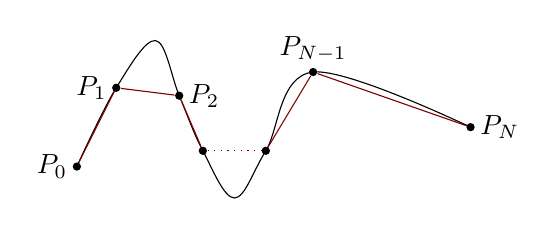
\begin{tikzpicture}
        \node [circ] (0) at (0, 0) {};
        \node [circ] (1) at (0.5, 1) {};
        \node [circ] (2) at (1.3, 0.9) {};
        \node [circ] (3) at (1.6, 0.2) {};
        \node [circ] (4) at (2.4, 0.2) {};
        \node [circ] (5) at (3, 1.2) {};
        \node [circ] (6) at (5, 0.5) {};
    
        \node [left] at (0) {$P_0$};
        \node [left] at (1) {$P_1$};
        \node [right] at (2) {$P_2$};
        \node [above] at (5) {$P_{N - 1}$};
        \node [right] at (6) {$P_N$};
    
        \draw plot [smooth, tension=0.6] coordinates {(0) (1) (1, 1.6) (2) (3) (2, -0.4) (4) (5) (6)};
        \draw [mred] (0) -- (1) -- (2) -- (3);
        \draw [mred, dotted] (3) -- (4);
        \draw [mred] (4) -- (5) -- (6);
      \end{tikzpicture}
    \end{center}
\end{frame}

\begin{frame}{Length of curve}
    \begin{defi}[Length of curve]
      The length of a curve $\Gamma: [a, b] \to \R^n$ is
      \[
        \ell = \sup_{\mathcal{D}} S_{\mathcal{D}},
      \]
      if the supremum exists.
    \end{defi}
    Alternatively, if we let
    \[
      \mathrm{mesh}(\mathcal{D})= \max_i (t_i - t_{i - 1}),
    \]
    then if $\ell$ exists, then we have
    \[
      \ell = \lim_{\mathrm{mesh}(\mathcal{D}) \to 0} s_{\mathcal{D}}.
    \]
\end{frame}

\subsection{The way to calculate length of curve}

\begin{frame}{How to calculate length of curve?}
    \begin{prop}
      If $\Gamma$ is continuously differentiable (i.e.\ $C^1$), then the length of $\Gamma$ is given by
      \[
        \length(\Gamma) = \int_a^b \|\Gamma'(t)\|\;\d t.
      \]
    \end{prop}
\end{frame}

\begin{frame}{Proof}
    To simplify notation, we assume $n = 3$. However, the proof works for all possible dimensions. We write
      \[
        \Gamma(t) = (f_1(t), f_2(t), f_3(t)).
      \]
      For every $s \not= t \in [a, b]$, the mean value theorem tells us
      \[
        \frac{f_i(t) - f_i(s)}{t - s} = f'_i (\xi_i)
      \]
      for some $\xi_i \in (s, t)$, for all $i = 1, 2, 3$.
\end{frame}

\begin{frame}{Proof}
    Now note that $f_i'$ are continuous on a closed, bounded interval, and hence uniformly continuous. For all $\varepsilon \in 0$, there is some $\delta > 0$ such that $|t - s| < \delta$ implies
          \[
            |f_i'(\xi_i) - f'(\xi)| < \frac{\varepsilon}{3}
          \]
          for all $\xi \in (s, t)$. Thus, for any $\xi \in (s, t)$, we have
          \[
            \left\|\frac{\Gamma(t) - \Gamma(s)}{t - s} - \Gamma'(\xi)\right\| = \left\|\begin{pmatrix}f'_1(\xi_1)\\ f'_2(\xi_2)\\ f'_3(\xi_3)\end{pmatrix} - \begin{pmatrix}f'_1(\xi)\\ f'_2(\xi)\\ f'_3(\xi)\end{pmatrix}\right\| \leq \frac{\varepsilon}{3} + \frac{\varepsilon}{3} + \frac{\varepsilon}{3} = \varepsilon.
          \]
          In other words,
          \[
            \|\Gamma(t) - \Gamma(s) - (t - s) \Gamma'(\xi)\| \leq \varepsilon(t - s).
          \]
          We relabel $t = t_i$, $s = t_{i - 1}$ and $\xi = \frac{s + t}{2}$.
\end{frame}

\begin{frame}{Proof}
    Using the triangle inequality, we have
  \begin{multline*}
    (t_i - t_{i - 1}) \left\|\Gamma'\left(\frac{t_i + t_{i - 1}}{2}\right)\right\| - \varepsilon(t_i - t_{i - 1}) < \|\Gamma(t_i) - \Gamma(t_{i - 1})\| \\
    < (t_i - t_{i - 1}) \left\|\Gamma'\left(\frac{t_i + t_{i - 1}}{2}\right)\right\| + \varepsilon(t_i - t_{i - 1}).
  \end{multline*}
  Summing over all $i$, we obtain
  \begin{multline*}
    \sum_i (t_i - t_{i - 1}) \left\|\Gamma'\left(\frac{t_i + t_{i - 1}}{2}\right)\right\| - \varepsilon(b - a) < S_{\mathcal{D}}\\
    < \sum_i (t_i - t_{i - 1}) \left\|\Gamma'\left(\frac{t_i + t_{i - 1}}{2}\right)\right\| + \varepsilon(b - a),
  \end{multline*}
  which is valid whenever $\mathrm{mesh}(\mathcal{D}) < \delta$.
\end{frame}

\begin{frame}{Proof}
    Since $\Gamma'$ is continuous, and hence integrable, we know
  \[
    \sum_i (t_i - t_{i - 1}) \left\|\Gamma'\left(\frac{t_i + t_{i - 1}}{2}\right)\right\| \to \int_a^b \|\Gamma'(t)\|\;\d t
  \]
  as $\mathrm{mesh}(\mathcal{D}) \to 0$, and
  \[
    \length(\Gamma) = \lim_{\mathrm{mesh}(\mathcal{D}) \to 0} S_\mathcal{D} = \int_a^b \|\Gamma'(t)\|\;\d t.\qedhere
  \]
\end{frame}

\begin{frame}[allowframebreaks]{References}
    \bibliography{refs}
    \bibliographystyle{abbrv}
    \nocite{*}
\end{frame}

% normal frame
% \section{Bayesian Statistics Tutorial}
% \subsection{}
% \begin{frame}
%     \frametitle{Basics}
%     conditional probabilities:
%     $$
%     p(x|y) \coloneqq \frac{p(x,y)}{p(y)}
%     $$
%     the joint probalility of $x$ and $y$:
%     $$
%     p(x,y)=p(x|y)p(y)=p(y|x)p(x)
%     $$

%     \begin{block}{Theorem: Bayes Rule}
%     Denote by X and Y random variables then the following holds
%     $$
%     p(y|x)=\frac{p(x|y)p(y)}{p(x)}
%     $$
%     \end{block}

% \end{frame}

% \begin{frame}
%     \frametitle{An Example}

%     \begin{parchment}[Question]
%         Assume that a patient would like to have such a test carried out on him. The physician recommends a test which is guaranteed to detect HIV-positive whenever a patient is infected. On the other hand, for healthy patients it has a $1\%$ error rate. That is, with probability 0.01 it diagnoses a patient as HIV-positive even when he is, HIV-negative. \uwave{Moreover, assume that $0.15\%$ of the population is infected.}
%         \\[1ex]
%         Now the patient has the test carried out and the test returns HIV-negative. In this case, logic implies that he is healthy, since the test has $100\%$ detection rate. In the converse case things are not quite as straightforward.
%         \\[1ex]
%         So what's the $p(X = \mathtt{HIV+}|T = \mathtt{HIV+})$?
%     \end{parchment}
    
% \end{frame}

% \begin{frame}
%     \frametitle{An Example}

%     \center{
%     \begin{tabular}{ c | c c }
%         $p(t|x)$ & $X = \mathtt{HIV-}$ & $X=\mathtt{HIV+}$ \\
%         \hline
%         $T=\mathtt{HIV-}$ & 0.99 & 0 \\
%         $T=\mathtt{HIV+}$ & 0.01 & 1
%     \end{tabular}
%     }

%     $$
%     p(X = \mathtt{HIV+}) = 0.0015
%     $$
% \end{frame}

% \begin{frame}
%     \frametitle{An Example}

%     By Bayes rule we may write
%     $$
%     p(X = \mathtt{HIV+}|T=\mathtt{HIV+}) = \frac{p(T=\mathtt{HIV+}|X=\mathtt{HIV+})p(X=\mathtt{HIV+})}{p(T=\mathtt{HIV+})}
%     $$

%     While we know all terms in the numerator, $p(T = \mathtt{HIV+})$itself is unknown. That said, it can be computed via
%     \begin{align}
%     \nonumber p(T=\mathtt{HIV+}) &= \sum_{x \in \{\mathtt{HIV+}, \mathtt{HIV-}\}}p(T=\mathtt{HIV+},x) \\
%     \nonumber &= \sum_{x \in \{\mathtt{HIV+}, \mathtt{HIV-}\}}p(T=\mathtt{HIV+}|x)p(x) \\
%     \nonumber &= 1.0 \cdot 0.0015 + 0.01 \cdot 0.9985
%     \end{align}

%     Substituting back into the conditional expression yields
%     $$
%     p(X = \mathtt{HIV+}|T=\mathtt{HIV+}) = \frac{1.0 \cdot 0.0015}{1.0 \cdot 0.0015 + 0.01 \cdot 0.9985} = 0.1306
%     $$

% \end{frame}


% \begin{frame}
%     \frametitle{How can we improve the diagnosis}

%     % Define block styles
%     \tikzset{
%         grayCircle/.style = {
%             draw,
%             circle,
%             node distance=2.5cm,
%             minimum size=1.5cm,
%             fill=black!20
%         }
%     }

%     \center
%     \begin{tikzpicture}
%         \node[grayCircle] (age) {age};
%         \node[grayCircle, right of=age, style={fill=none}] (x) {x};
%         \node[grayCircle, right of=x, yshift=1.25cm] (t1) {test 1};
%         \node[grayCircle, below of=t1] (t2) {test 2};
%         \draw[->, >=latex] (age) -- (x);
%         \draw[->, >=latex] (x) -- (t1);
%         \draw[->, >=latex] (x) -- (t2);
%     \end{tikzpicture}

%     \begin{figure}
%         \caption{A graphical description of our HIV testing scenario. Knowing the age of the patient influences our prior on whether the patient is HIV positive (the random variable X). The outcomes of the tests 1 and 2 are independent of each other given the status X. We observe the shaded random variables (age, test 1, test 2) and would like to infer the un-shaded random variable X.}
%     \end{figure}

% \end{frame}


% \begin{frame}
%     \frametitle{How can we improve the diagnosis}

%     \begin{parchment}[Including additional observed random variables]
%     One way is to obtain further information about the patient and to use this in the diagnosis. For instance, information about his age is quite useful. Suppose the patient is 35 years old. In this case we would want to compute $p(X = \mathtt{HIV+}|T = \mathtt{HIV+}, A = 35)$ where the random variable A denotes the age.
%     \end{parchment}

%     The corresponding expression yields:
%     $$
%     \frac{p(T=\mathtt{HIV+}|X=\mathtt{HIV+},A)p(X=\mathtt{HIV+}|A)}{p(T=\mathtt{HIV+}|A)}
%     $$
% \end{frame}


% \begin{frame}
%     \frametitle{How can we improve the diagnosis}

%     We may assume that the test is independent of the age of the patient, i.e.
%     $$
%     p(t|x,a) = p(t|x)
%     $$

%     What remains therefore is $p(X = \mathtt{HIV+}|A)$. Recent US census data pegs this number at approximately $0.9\%$. 
%     \begin{align}
%     \nonumber & p(X = \mathtt{H+}|T = \mathtt{H+}, A) = \frac{p(T=\mathtt{H+}|X=\mathtt{H+},A)p(X=\mathtt{H+}|A)}{p(T=\mathtt{H+}|A)} \\
%     \nonumber &= \frac{p(T=\mathtt{H+}|X=\mathtt{H+},A)p(X=\mathtt{H+}|A)}{p(T=\mathtt{H+}|X=\mathtt{H+},A)p(X=\mathtt{H+}|A) + p(T=\mathtt{H+}|X=\mathtt{H-},A)p(X=\mathtt{H-}|A)} \\
%     \nonumber & = \frac{p(T=\mathtt{H+}|X=\mathtt{H+})p(X=\mathtt{H+}|A)}{p(T=\mathtt{H+}|X=\mathtt{H+})p(X=\mathtt{H+}|A) + p(T=\mathtt{H+}|X=\mathtt{H-})p(X=\mathtt{H-}|A)} \\
%     \nonumber & = \frac{1 \cdot 0.009}{1 \cdot 0.009 + 0.01 \cdot 0.991} = 0.48
%     \end{align}

% \end{frame}


% \begin{frame}
%     \frametitle{How can we improve the diagnosis}

%     \begin{parchment}[Multiple measurements]
%     A second tool in our arsenal is the use of multiple measurements. After the first test the physician is likely to carry out a second test to confirm the diagnosis. We denote by $T_1$ and $T_2$ (and $t_1$,$t_2$ respectively) the two tests. Obviously, what we want is that $T_2$ will give us an "independent" second opinion of the situation.
%     \\[2ex]
%     What we want is that the diagnosis of $T_2$ is independent of that of $T_2$ given the health status X of the patient. This is expressed as
%     $$
%     p(t_1,t_2|x) = p(t_1|x)p(t_2|x)
%     $$
%     which are commonly referred to as \uwave{conditionally independent}.

%     \end{parchment}
% \end{frame}

% \begin{frame}
%     \frametitle{How can we improve the diagnosis}

%     we assume that the statistics for $T_2$ are given by
%     \center{
%     \begin{tabular}{ c | c c }
%         $p(t_2|x)$ & $X = \mathtt{HIV-}$ & $X=\mathtt{HIV+}$ \\
%         \hline
%         $T_2=\mathtt{HIV-}$ & 0.95 & 0.01 \\
%         $T_2=\mathtt{HIV+}$ & 0.05 & 0.99 
%     \end{tabular}
%     }

%     \flushleft
%     for $t_1 = t_2 = \mathtt{HIV+}$ we have
%     \begin{align}
%     \nonumber & p(X=\mathtt{H+}|T_1=\mathtt{H+},T_2=\mathtt{H+}) \\
%     \nonumber &= \frac{p(T_1=\mathtt{H+}, T_2=\mathtt{H+}|X=\mathtt{H+})p(X=\mathtt{H+}|A)}{p(T_1=\mathtt{H+}, T_2=\mathtt{H+}|A)} \\
%     \nonumber &= p(T_1=\mathtt{H+}|X=\mathtt{H+})p(T_2=\mathtt{H+}|X=\mathtt{H+})p(X=\mathtt{H+}|A) \;/ \\
%     \nonumber & p(T_1=\mathtt{H+}|X=\mathtt{H+})p(T_2=\mathtt{H+}|X=\mathtt{H+})p(X=\mathtt{H+}|A) \\
%     \nonumber & + p(T_1=\mathtt{H+}|X=\mathtt{H-})p(T_2=\mathtt{H+}|X=\mathtt{H-})p(X=\mathtt{H-}|A) \\
%     % \nonumber & p(T_{1,H+}|X_{H+})p(T_{2,H+}|X_{H+})p(X_{H+}|A) \\
%     % \nonumber & + p(T_{1,H+}|X_{H-})p(T_{2,H+}|X_{H-})p(X_{H-}|A) \\
%     \nonumber &= \frac{1 \cdot 0.99 \cdot 0.009}{1 \cdot 0.99 \cdot 0.009 + 0.01 \cdot 0.05 \cdot 0.991} = 0.95
%     \end{align}
% \end{frame}

\end{document}